\documentclass{article}
    
\usepackage{Haust2017skil}
\usepackage{caption}
\usepackage{subcaption}

\title{Stærðfræðimynstur í tölvunarfræði \\ Skilaverkefni 11}
\author{}

\begin{document}
\maketitle

Skila skal þessu verkefni á vefnum \href{https://gradescope.com/courses/9487}{Gradescope}. Aðgangskóði fyrir námskeiðið er \textbf{9N834D}.
Þeim má skila sem einstaklingar eða \emph{tvö og tvö saman}.

Gradescope tekur við .pdf skjölum. Frágangur á þeim skiptir máli. Þau skulu vera hreinskrifuð í tölvu. 
%Kerfi eins og \LaTeX, Google Docs og Microsoft Word geta búið til .pdf skjöl. 
Mikilvægt er að merkja á hvaða blaðsíðu .pdf skjalsins hver lausn kemur fyrir, ekki er hægt að gera ráð fyrir að dæmatímakennarar fari yfir ómerkt dæmi.

Telji nemandi að mistök hafi verið gerð við yfirferð skal tilkynna slíkt með tölvupósti til dæmatímakennara. Nálgast má lista yfir hvaða dæmatímakennari fór yfir hvaða dæmi á Piazza-vef námskeiðsins.
\section{Kafli 10.4}

\question Útskýrið af hverju þessi net hafa engar brýr.

\begin{itemize}
 \item[b)] $W_n$ með $n \geq 3$
 \item[c)] $K_{m,n}$ með $m \geq 2, n \geq 2$
\end{itemize}

\textbf{Í bók:} \quad Hluti af 10.4.48 í International/Icelandic, 10.5.34 í Global

\question Gömul þraut snýst um raunir bónda nokkurs við að ferja úlf, geit og kálpoka yfir á. Bóndinn á einungis lítinn bát, svo hann getur einungis flutt einn hlut eða eina skepnu yfir í einu, auk sjálfs sín. Bóndinn getur ferjað hlutina fram og til baka að vild, en ekki er hægt að skilja geitina eina eftir með kálpokanum (því þá étur geitin kálið) og ekki er hægt að skilja úlfinn eftir eftirlitslausan með geitinni (því þá étur úlfurinn geitina).

Lýsum mögulegu ástandi í þrautinni með röðuðu pari. Til dæmis, þá er $(BG,UK)$ það ástand þar sem bóndinn og geitin eru á fyrri bakkanum en úlfurinn og kálpokinn á seinni bakkanum. Notum táknið $\emptyset$ til að lýsa því að ekkert sé á bakka, svo $(BUGK, \emptyset)$ er upphafsástandið.

Finnið öll ástönd þrautarinnar þar sem hvorki geitin né kálið er étið. Látið síðan hvert ástand tákna hnút í neti og tengið hnútana saman sé mögulegt að færast á milli ástandanna með einni bátsferð.

Teiknið netið og sýnið veg í netinu sem táknar lausn á þrautinni.

\paragraph{Í bók:} Byggt á 10.4.64 í International/Icelandic, 10.4.50 í Global

\section{Kafli 10.5}

\question 

\paragraph{(Ísl)} Er hægt að ganga nákvæmlega einu sinni yfir hverja brú í þessari borg og enda aftur á sama stað og viðkomandi byrjaði á? Rökstyðjið með netaframsetningu.

\paragraph{(En)} Can someone cross all the bridges shown in this map exactly once and return to the starting point? Demonstrate using a graph representation.

\begin{center}
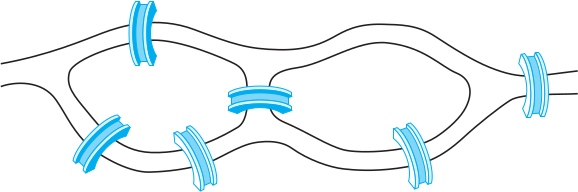
\includegraphics[width=0.5\textwidth]{not-konigsberg-graph}
\end{center}

\paragraph{Í bók:} Exercise 10.5.10, ekki til staðar í Global

\question Fyrir hvaða gildi á $n$ hafa eftirfarandi net Euler-rás? En Hamilton-rás? Útskýrið.

\begin{itemize}
 \item[a)] $K_n$
 \item[b)] $C_n$
\end{itemize}

\paragraph{Í bók:} Hluti af 10.5.26 og 10.5.44 í International/Icelandic, 10.5.16 og 10.5.24 í Global.

\question Finnið léttasta veg á milli gefnu borganna í eftirfarandi neti. Sýnið vegina og heildarþyngdir þeira.

\begin{center}
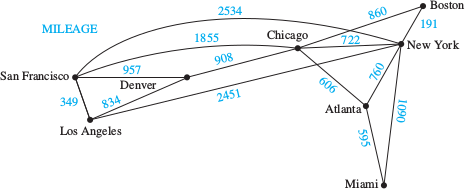
\includegraphics[width=0.6\textwidth]{graph-weighted-mileage}
\end{center}

\begin{itemize}
 \item[b)] San Francisco og Los Angeles
 \item[c)] Miami og Denver
\end{itemize}

\paragraph{Í bók:} Hluti af 10.6.8 í International/Icelandic, 10.6.5 í Global

\paragraph{Ábending:} Þetta er frábært tækifæri til æfingar í reikniriti Dijkstra.

\question 

\paragraph{(Ísl)} Hafi engir tveir leggir í vegnu samanhangandi neti með a.m.k. þrjá hnúta og þrjá leggi sömu þyngd, er alltaf einn léttasti vegur á milli tveggja hnúta?

Ef ekki, sýnið mótdæmi. Sé svo, sýnið fram á það.

\paragraph{(En)} Is a shortest path between two vertices in a connected, weighted graph with at least three vertices and three edges unique if the weights of edges are distinct?

If not, present a counterexample. If so, demonstrate it.


\end{document}
